%%%%%%%%%%%%%%%%%%%%%%%%%%%%%%
% LATEX-TEMPLATE TECHNICAL REPORT
%-------------------------------------------------------------------------------
% Voor informatie over het technisch rapport, zie
% http://practicumav.nl/onderzoeken/rapport.html
% Voor readme en meest recente versie van het template, zie
% https://gitlab-fnwi.uva.nl/informatica/LaTeX-template.git
%%%%%%%%%%%%%%%%%%%%%%%%%%%%%%

%-------------------------------------------------------------------------------
%	PACKAGES EN DOCUMENT CONFIGURATIE
%-------------------------------------------------------------------------------

\documentclass{uva-inf-article}
\usepackage[utf8]{inputenc}
\usepackage[english]{babel}

\usepackage[
backend=biber,
style=numeric,
citestyle=numeric 
]{biblatex}

\addbibresource{citations.bib} %Imports bibliography file

% Relevant voor refereren vanaf blok 5
%\usepackage[style=authoryear-comp]{biblatex}
%\addbibresource{citations.bib}

%-------------------------------------------------------------------------------
%	GEGEVENS VOOR IN DE TITEL
%-------------------------------------------------------------------------------

% Vul de naam van de opdracht in.
\assignment{Software Process}
% Vul het soort opdracht in.
\assignmenttype{Report}
% Vul de titel van de eindopdracht in.
\title{Assignment 2}

% Vul de volledige namen van alle auteurs in.
\authors{Piotr Kosytorz}
% Vul de corresponderende UvAnetID's in.
\uvanetids{UvAnetID 11876964}

% Vul altijd de naam in van diegene die het nakijkt, tutor of docent.
\tutor{drs. Hans Dekker}
% Vul eventueel ook de naam van de docent of vakcoordinator toe.
\docent{}
% Vul hier de naam van de PAV-groep  in.
\group{}
% Vul de naam van de cursus in.
\course{Software Process}
% Te vinden op onder andere Datanose.
\courseid{}

% Dit is de datum die op het document komt te staan. Standaard is dat vandaag.
\date{\today}


\usepackage{rotating}
\usepackage{booktabs}

%-------------------------------------------------------------------------------
%	VOORPAGINA
%-------------------------------------------------------------------------------

\begin{document}
\maketitle

%-------------------------------------------------------------------------------
%	INHOUDSOPGAVE EN ABSTRACT
%-------------------------------------------------------------------------------

\tableofcontents

\section{Best practices}\label{best-practices}

In an article from 2000 by James Salapatas for the Project Management Institute, nine best practices for achieving success in a project are provided\cite{salapatas2000}: 

\begin{enumerate}
\item Defined Life Cycle and Milestones \\
\textit{Organizations need to map and define phases, deliverables, key milestones and sufficiency criteria for each group involved in the project.}\cite{salapatas2000}

\item Stable Requirements and Scope \\
\textit{Effective project management requires that project requirements, objectives and scope be documented and become stabilized at some point early in the project life cycle.}\cite{salapatas2000}

\item Defined Organization, Systems, and Roles \\
\textit{In any organization projects must have defined roles for the project manager, functional managers and project team members. Accountabilities must be identified for all.}\cite{salapatas2000}

\item Quality Assurance \\
\textit{Quality on projects requires the identification of standards and criteria to be set in each phase of the project life cycle for both the product and the process. Quality means making and meeting agreed to commitments with a constant eye for improvement.}\cite{salapatas2000}

\item Planned Commitments \\
\textit{Plans must be based upon the process capability of the organization and not upon wishful thinking. It is common to see wishful project schedules built upon a ``house of cards'' where sufficient resources are not available. Plans must be more than schedules in that they address all nine elements of the project management process.}\cite{salapatas2000}

\item Tracking and Variance Analysis \\
\textit{Projects should be managed using an exception process in which deviations from plans are reported and resolved.}\cite{salapatas2000}

\item Corrective Action Decisions \\
\textit{When variances from plan are detected, the default assumption is that the team or functional groups will work to put the project back on track. Without a clear procedure corrective action can have many outcomes, not all consistent with corporate objectives.}\cite{salapatas2000}

\item Escalation and Issue Management \\
\textit{An effective escalation procedure requires issues and problems to be worked first by the lowest appropriate level. If the issue cannot be resolved and closed, then it must be elevated to the next highest organizational level, and so on until the issue is closed. }\cite{salapatas2000}

\item Work Authorization and Change Control \\
\textit{Late changes in projects are a major source of disruption that lead to schedule slippage, cost overruns, insertion of defects and rework. A formal system of change control and change management must be in place. Changes caused by scope creep must be resisted and change control is needed to prevent these problems.}\cite{salapatas2000}

\end{enumerate}

In my report on Methods, I will be referring to these nine best practices.

\section{Methods}

\subsection{Waterfall (1970)}\label{waterfall}

Waterfall is a sequentially structured project management methodology. According to Royce \cite{Royce1970}, the methodology can
be described as a sequence of the following phases:

\begin{enumerate}

\item
  System requirements
\item
  Software requirements
\item
  Analysis
\item
  Program design
\item
  Coding
\item
  Testing
\item
  Operations
\end{enumerate}

Royce draws attention to two very important aspects of waterfall
methodology in its starting phases: documentation and project knowledge.
As he says, \emph{During the early phase of software development the
documentation is the specification and is the design.}\cite{Royce1970} Documentation is thus the backbone of project management. Writing documentation guarantees early testing of (errors) in the design and concept: \emph{Without good documentation every mistake,
large or small, is analysed by one man who probably made the mistake in the first place because
he is the only man who understands the program area}\cite{Royce1970}

The second thing Royce mentions is project knowledge: there should be at least one person that has a deep understanding of the whole system. This knowledge must be the exhaustively put into documentation. Each project phase must deliver appropriate documentation: \emph{At least one person must have a deep understanding of the system which comes partially from having had to write an overview document}\cite{Royce1970}

Waterfall as methodology sets up a clear structure in project
management. Each proceeding phase is a logical result of the previous
one.

Waterfall seems a good solution to projects which requirements can be fully determined from the beginning. Unfortunately, there is very little (or actually none) space for requirements change during the project. Royce gives examples of systems that take 12 months to develop.

Due to the fact that in waterfall, proceeding from one phase another
requires an extended amount of work and documentation, every change in
requirements would heavily disturb the process.

Waterfall is a good fit for highly specialized projects, that stay conservative in their requirements and don't have much rotation of personnel in their development teams. 

Another aspect in favour of the statement that Waterfall is more a fit for projects that are conservative in their requirements is the fact, that Royce mentions: \emph{If the computer program in question is being developed for the first time, arrange
matters so that the version finally delivered to the customer for operational deployment is actually the second
version insofar as critical design/operations areas are concerned.}\cite{Royce1970}

According to the list of best practices from chapter \ref{best-practices}, waterfall is missing Corrective Action Decisions and Work Authorization and Change Control, as waterfall is designed to be sequential, and there is no formal mechanism for re-iterating parts of the project.  

\subsection{Scrum (1986)}
\begin{figure}
 \caption{The Scrum Framework\cite{scrum2013scrum}}
 \centering 
 \makebox[\textwidth]{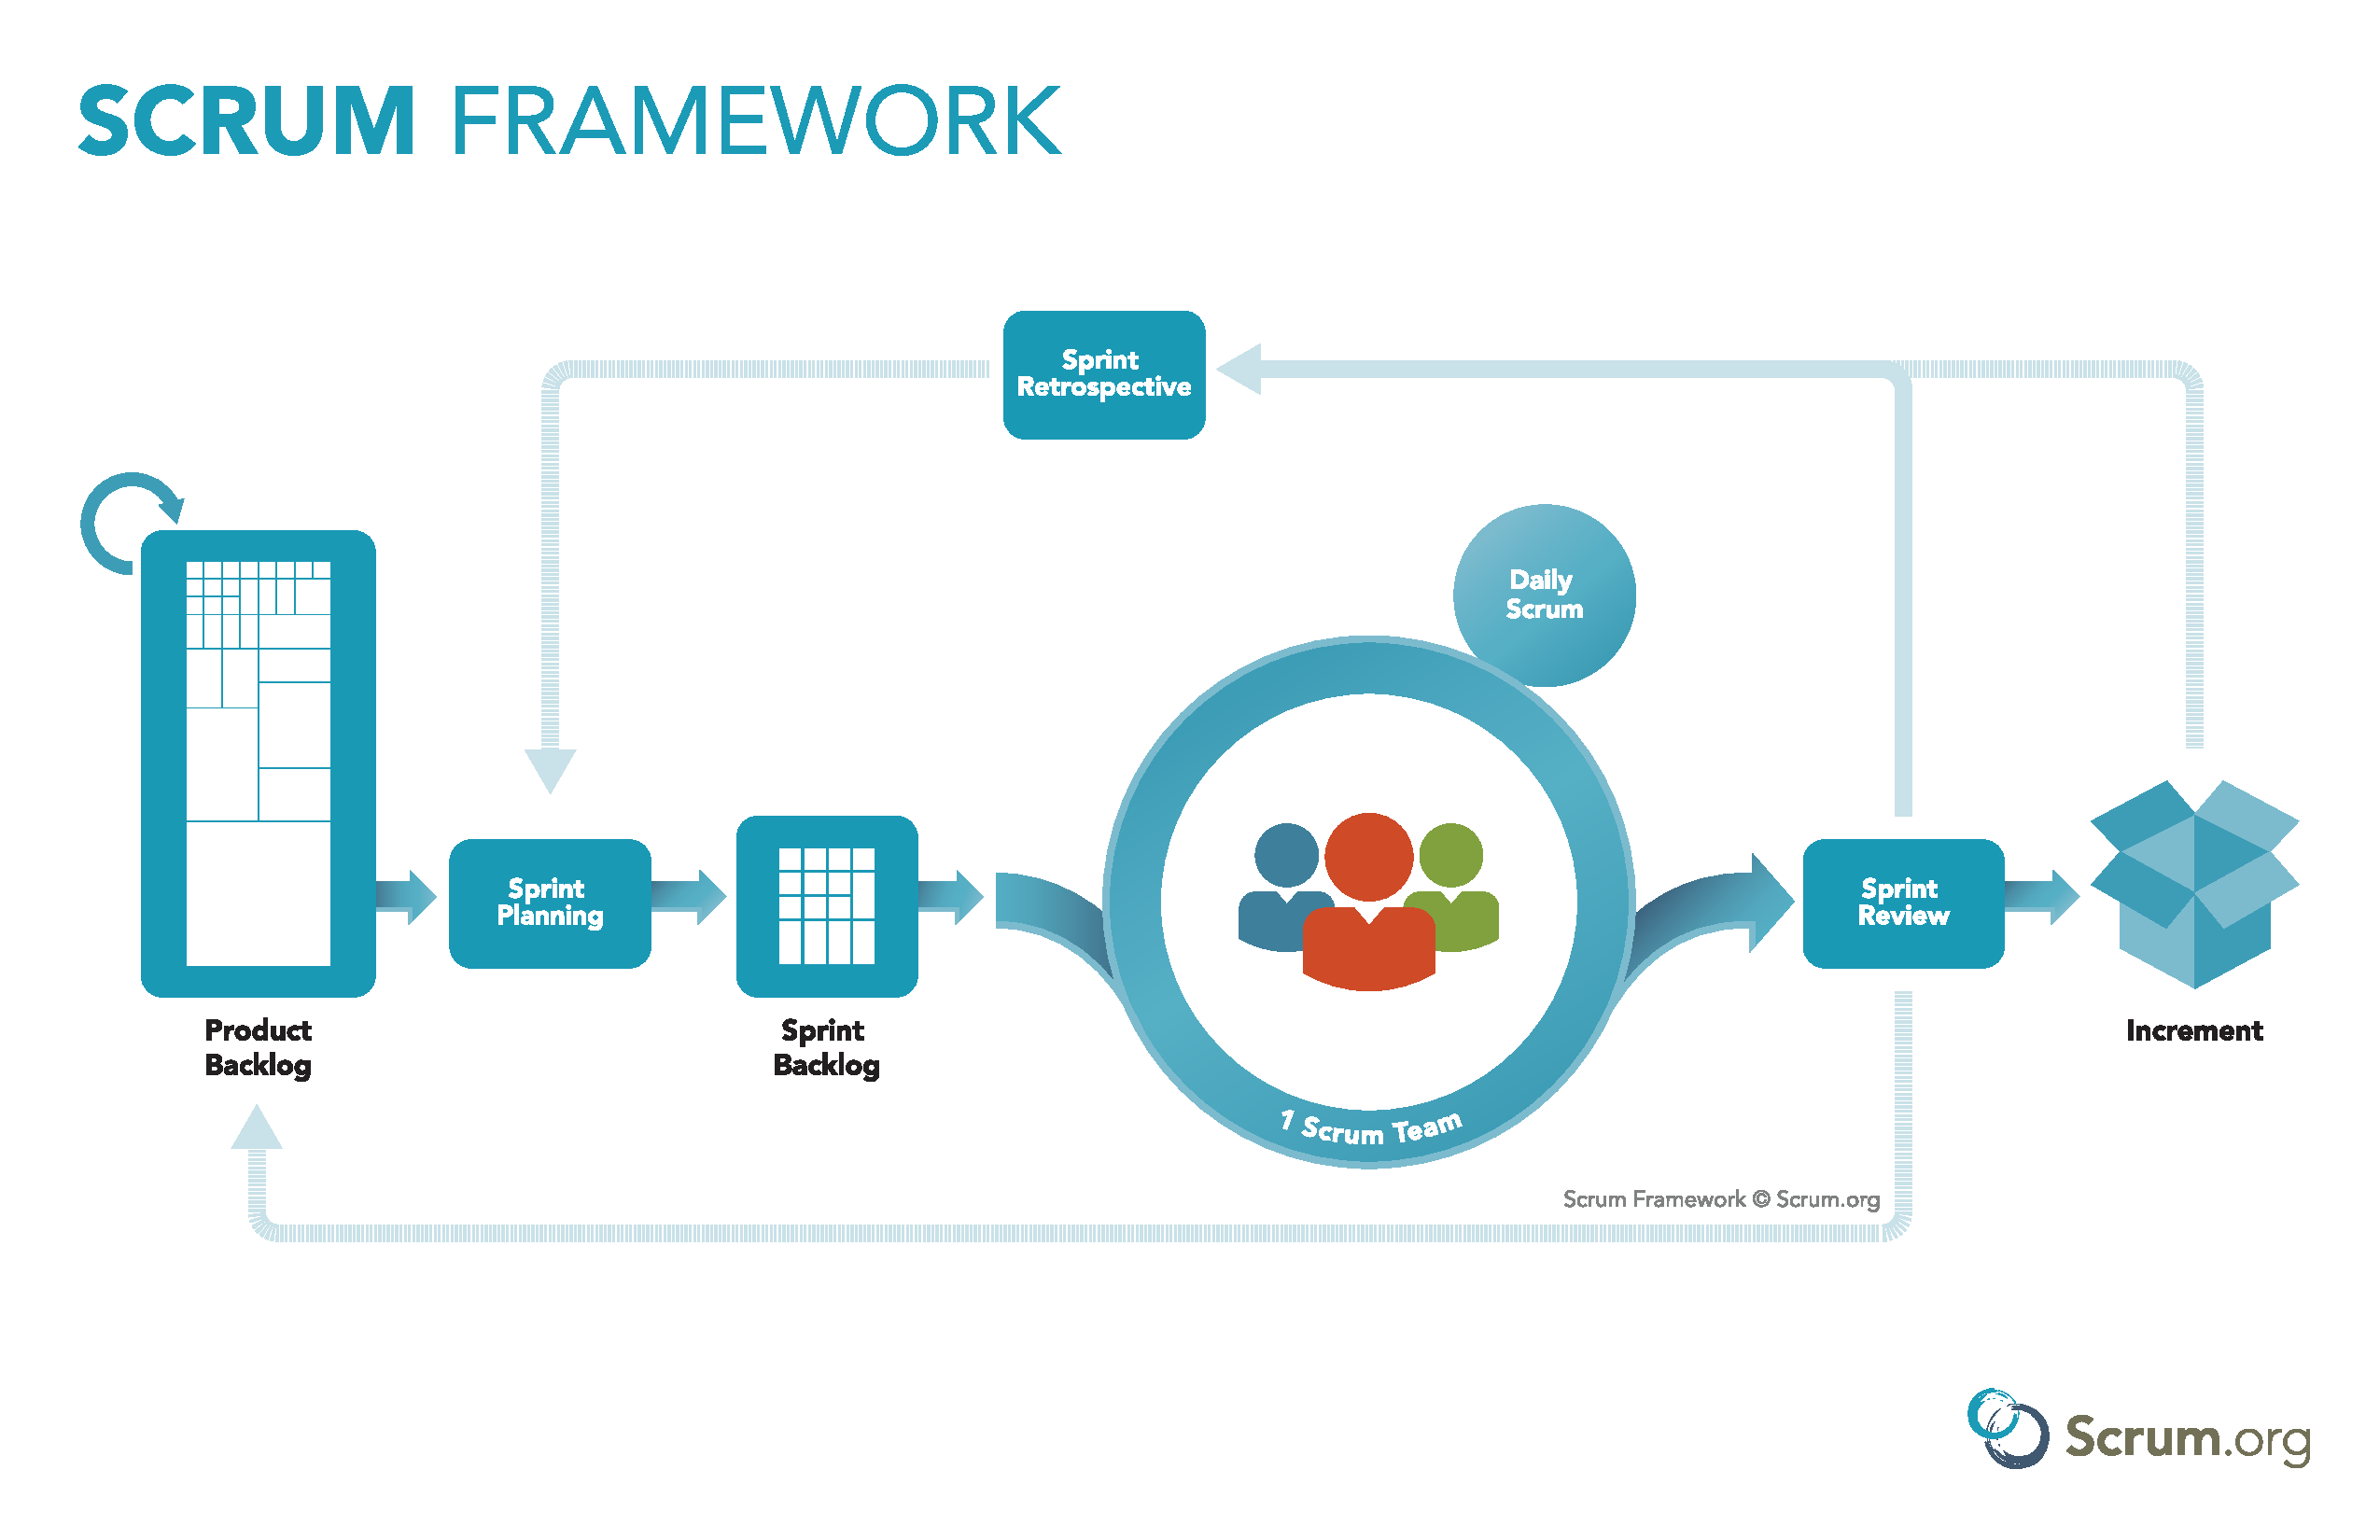
\includegraphics[width=\textwidth]{scrum.pdf}}
\end{figure}

According to Schwaber\cite{schwaber2011scrum} \emph{Scrum is a framework for developing and sustaining complex products}.\cite{schwaber2011scrum}

Scrum consists the following elements:

\begin{itemize}

\item
  Product: \emph{what has to be produced}

  \begin{itemize}
  
  \item
    Backlog: \emph{list of elements that will eventually collectively
    produce the end product}
  \end{itemize}
\item
  Sprint: \emph{a sub-project limited by time with a precisely
  determined output}

  \begin{itemize}
  
  \item
    Planning
  \item
    Backlog: \emph{list of tasks in current sprint (a subset of product
    backlog)}
  \item
    Review: \emph{analysis of the meaning and fitness of the current
    sprint in relation to the whole product}
  \item
    Retrospective: \emph{analysis of what have we done wrong, what can
    we do better next time}
  \end{itemize}
\item
  Scrum team

  \begin{itemize}
  
  \item
    Product Owner: \emph{Domain specialist}
  \item
    Development Team \emph{The blue collar workers}
  \item
    Scrum Master: \emph{Judge in the ring: makes sure that there is a
    healthy relationship between the product owner and the development
    team, and that they follow the rules.}
  \end{itemize}
\item
  Daily scrum: \emph{a 15-minute time-boxed daily meeting/discussion}
\item
  Increment: \emph{A finished spring that builds up the final product.}
\end{itemize}

Scrum introduces a lot of flexibility in project management and
development. The work is divided into manageable chunks. There is always
someone who knows what has to be achieved in the project (Product
Owner), and someone who takes care of the team and makes sure that the
rules are being played fair (Scrum Master).

Scrum can be applied to both: big and small projects. It allows project
adaptation, thus change in requirements is taken into account.

In the terms of best practices introduced in chapter \ref{best-practices}, scrum fulfils all the criteria, if done correctly. In practice Stable Requirements and Scope can be a weak point, because as every Agile method, scrum puts pressure more on single iteration (sprints) than on a holistic vision of the project.

\subsection{Agile (2001)}\label{agile}

Agile manifesto\cite{fowler2001agile}:

\begin{itemize}
\item
  \textbf{Individuals and interactions} over processes and tools
\item
  \textbf{Working software} over comprehensive documentation
\item
  \textbf{Customer collaboration} over contract negotiation
\item
  \textbf{Responding to change} over following a plan
\end{itemize}

Agile as a philosophy puts pressure on the value of human and practical aspects of software development, rather than of a formalized path to follow. 

Salapatas' best practices are not applicable here.

\subsection{RUP (2003)}\label{rup}

Rational Unified Process is another software development framework with another look into the problem of project development. The main focus of the framework is to ensure that everyone in the team knows what to do, therefore it is based on three elements:

\begin{itemize}
\item
  Roles (who)
\item
  Work products (what)
\item
  Tasks (how)
\end{itemize}

Shortly: \textbf{Who} produces \textbf{what}, and \textbf{how} does he
do that?\cite{wiki:Rational_Unified_Process}\cite{powell-morse_2017}
\\\\
On the other hand, RUP tries to apply the best of both: Waterfall and
Scrum. It consists of four phases:

\begin{itemize}
\item
  Inception,
\item
  Elaboration,
\item
  Construction,
\item
  Transition,
\end{itemize}

where all six ``engineering disciplines'' are present, but with
different intensity according to different phases.

Within all the phases RUP introduces international development.

RUP seems like a good solution for big and highly skilled teams of
professionals within big organizations (like IBM itself).

RUP implements all of Salapatas' best practices.  

\subsection{Extreme Programming (2000)}\label{extreme-programming}

Extreme Programming is an Agile process, that focuses on:\cite{beck2004extreme}\cite{wiki:Extreme_programming}\cite{alliance_2018}

\begin{itemize}

\item
  delivering software (features) as soon as possible,
\item
  testing/gaining feedback from the customers as soon as possible,
\item
  delivering what you need when you need it, and only when you need it,
\item
  staying flexible to respond to changing requirements and technology,
\item
  enabling the teams to self-organize around the problem to solve it as
  efficiently as possible.
\end{itemize}

Extreme programming seems can be successfully applied in small teams
that do not require highly skilled programmers \cite{alliance_2018}. Start-up projects could benefit from this approach as well, since the request for requirements change there is high. XP, however, does not seem as a solution for big and highly specialized projects that require a holistic and deep understanding of the domain.

In terms of Salapatas' best practices XP is missing Stable Requirements and Scope and Defined Organization, Systems, and Roles.

\subsection{DevOps (2008)}\label{devops}

According to Wikipedia: \emph{DevOps (a clipped compound of
``development'' and ``operations'') is a software engineering culture
and practice that aims at unifying software development (Dev) and
software operation (Ops). The main characteristic of the DevOps movement
is to strongly advocate automation and monitoring at all steps of
software construction, from integration, testing, releasing to
deployment and infrastructure management. DevOps aims at shorter
development cycles, increased deployment frequency, and more dependable
releases, in close alignment with business objectives.}\cite{wiki:DevOps}

DevOps changes the way teams of specialists cooperate with each other.
This results in process change.

According to Amazon\cite{aws-devops}, the following are the DevOps best practices:

\begin{itemize}

\item
  Continuous Integration
\item
  Continuous Delivery
\item
  Microservices
\item
  Infrastructure as Code
\item
  Monitoring and Logging
\item
  Communication and Collaboration
\end{itemize}

\paragraph{What does DevOps change to Waterfall, Scrum, Agile, RUP, and
XP?}

DevOps introduces automation of repeatable processes, strong decoupling of projects and greater insight in software performance and software process. Linus Torvalds in his talk about Git at Goole \href{https://www.youtube.com/watch?v=4XpnKHJAok8}{link} said, that the speed of your tools (processes) changes, then the way you use them
changes as well. To me this is a great paraphrase of what DevOps does to software development methodologies - it changes the way we apply them. The focus is not so much laid on the interfaces between different phases of different methodologies, but rather on the core problems of software development and software quality itself.

\section{Discussion}

As Bethany Cartwright aptly states in her article\cite{cartwright_2015}: \textit{There are two main types of project management methodologies: waterfall and agile.} They differ a lot, and when looking at the time and circumstances of their publications, it is safe to say, that waterfall was and still is the way to go for bog projects that can be hold a conservative approach to their requirements. Since the beginning of the IT revolution, bigger and bigger presence of software in business and all kinds of devices, and especially since the Internet, waterfall had to make more and more place for agile. The rate of delivering software has rapidly increased in the last years. In the guest lectures by Amazon and Adyen, we have learned that they deploy their software even multiple times a day. Waterfall cannot be applied in such circumstances any more. 

When it comes to all the different Agile methods, like Scrum, XP, etc., the choice for specific method (or framework) is a matter of fitness for a specific project and team. 

The only exception is RUP, as a combination of best practices of both: Waterfall and Agile is is probably a great alternative for big-scale Waterfall projects that need a transition to a more agile approach.

Regardless of the choice of a method, the process does not guarantee a successful delivery of the end product. All of the discussed methods have their strong and weak sides, and they are only tools to improve the work flow.

\begin{table}[]
\centering
\caption{Methods trade-off}
\label{methods-trede-off}

\begin{tabular}{@{}lllllll@{}}
\toprule
Method/characteristic    & Waterfall & Scrum & Agile & RUP    & XP & DevOps \\ \midrule
Publication year         & 1970      & 1986  & 2001  & 2003   & 2000                & 2008   \\
Project time open/closed & closed    & open  & n.a.  & closed & open                & open   \\
Self-organization        & no        & yes   & yes   & no     & yes                 & yes    \\
Transparency             & no        & yes   & n.a.  & yes    & yes                 & yes    \\
Inspection               & no        & yes   & n.a.  & yes    & yes                 & yes    \\
Adaptation               & no        & yes   & yes   & yes    & yes                 & yes    \\
Iteration                & no        & yes   & yes   & yes    & n.a.                & yes    \\ \bottomrule
\end{tabular}
\end{table}

%-------------------------------------------------------------------------------
%	REFERENTIES
%-------------------------------------------------------------------------------

\printbibliography


\end{document}